\chapter{Thrust 0: \Cyclus Infrastructure Development}\label{chap:thrust0}

Under Thrust 0, the \Cyclus framework was advanced from a conceptual design to
a fully functional software tool.  As this project began, the fundamental
features of \Cyclus were in place, but it was far from a usable tool for fuel
cycle simulation.  Through the efforts of this project, \Cyclus emerged as a
more usable and stable software platform for nuclear fuel cycle analysis.  The
overarching goal was to provide maximum flexibility so that changes in fuel
cycle design did not require substantial retooling of the software.  Specific
design features that support this flexibility include:
\begin{enumerate}
\item \textbf{Modular design} to support extensibility with runtime swappable facility models.
\item \textbf{Agent-based approach} to incorporate social/behavior interaction models to govern how each facility interacts with others.
\item \textbf{Individual facility modeling} to allow each facility to operate in a distinct manner, allowing modeling of startup, shutdown and other disruptions.
\item \textbf{Discrete material tracking at the nuclide level} to capture the effects of individual facility performance and enable forensic tracking of material object ownership.
\item \textbf{Minimal physics assumptions} to enable different users to invoke low fidelity, systems level models or high fidelity, facility level models, or anything in between.
\end{enumerate}

Under this project, the \Cyclus effort developed into an \textit{ecosystem} composed of:
\begin{itemize}
\item an open source simulation kernel, known as \Cyclus,
\item many plug-in modules, each implementing a particular model for a
  facilty, institution or region, and known as \textit{archetypes}, and
\item an open source analysis and visualization tool, known as Cyclist.
\end{itemize}

The first section of this chapter will describe the fundamental design and
implementation of the \Cyclus kernel while the following section will describe
the infrastructure to support the development of new archetypes.

\section{Fundamental Design and Implementation} %%fundamentals paper

More details regarding the implementation and demonstration of the fundamental
design of the \Cyclus kernel are available in ref
\citeprod{huff-fundamentals}/.

\subsection{Modularity}

The modular nature of \Cyclus is a key element to its ability to remain
flexible, and also drives many subsequent design decisions.  The main goal of
this flexibility is to allow for the computational models that represent
individual agents (see Section \ref{sec:agents}) to be swapped easily, as a
user option.  Two specific advantages of this choice are that (a) individual
researchers can focus their efforts on new modules that match their expertise
and support their needs, and (b) the impact of changing modeling choices can
be explored in a consistent environment by swapping only one module at a time.

In it's purest expression, each module operates in a so-called
\textit{black-box} fashion.  That is, any single module has no knowledge of
the internal state or behavior of any other module and can only interact in a
narrowly defined and specific way.  In addition to imposing a number of
software engineering limitations on the implementation of the kernel and
archetypes, this design goal also requires careful design of that interaction
interface among the modules.

Figure \ref{fig:framework} illustrates this concept, indicating the different
\gls{API} for each type of agent, and the possibility of different
implementations in each case.  Different implementations of each type of
facility, for example, may use different models to describe the physics and/or
the interaction behavior of that facility.  These differences can represent
small perturbations from other implementations or entirely different
approaches, including wrapping other software.  Because the modules can be
swapped at runtime, without requiring the software to be recompiled, this also
facilitates different distribution modes for these modules, as shown in Figure
\ref{fig:modifiedopen}, including fully open source, export controlled, and/or
proprietary commercially licensed modules.

\begin{figure}[htbp]
\begin{center}
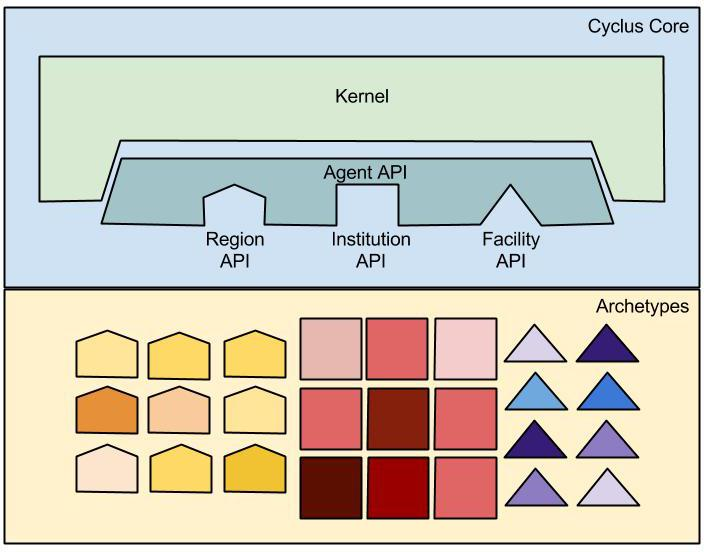
\includegraphics[width=0.7\columnwidth]{./images/framework}
\caption{The \Cyclus core provides \glspl{API} that abstract away the details in
the kernel and allow the archetypes to be loaded into the simulation in a modular
fashion.\cite{huff-fundamentals}}
\end{center}
\label{fig:framework}
\end{figure}

\begin{figure}[htbp]
\begin{center}
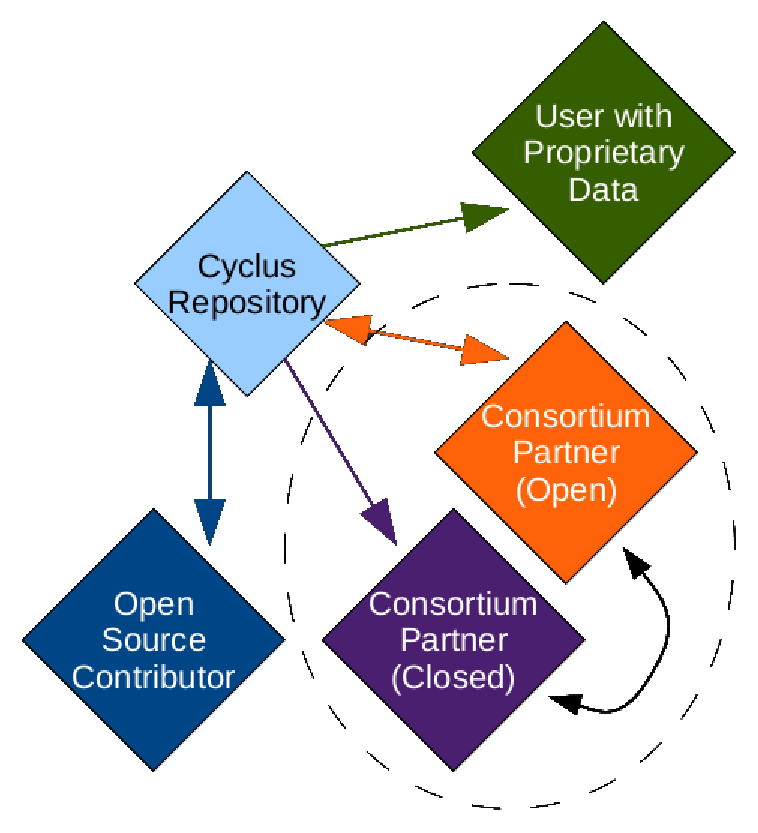
\includegraphics[width=0.5\columnwidth]{./images/modifiedopen.eps}
\caption{The \Cyclus framework enables fully open, partially open, and fully
closed collaborations\cite{carlsen_cyclus_2014}.}
\end{center}
\label{fig:modifiedopen}
\end{figure}


\subsection{Agent-based Paradigm}
\label{sec:abm}
% superior detail in capturing simulation dynamics
% more flexible control over behavior
% describe Region/Institution/Facility hierarchy
% note importance of generic resource exchange paradigm

\Cyclus implements an \acrlong{ABM} paradigm.  In addition to being a natural
consquence of the modularity described above, the \gls{ABM} paradigm is more
flexible and intuitive (from both a developer and user perspective) than the
system dynamic approach used in current simulators.  System dynamics is a
popular approach for modeling nuclear fuel cycles
\cite{jacobson_vision_2009,van_den_durpel_daness_2009,guerin_impact_2009,guerin_benchmark_2009}.
Formally however, system dynamics models are simply a strict subset of
agent-based models \cite{macal_agent-based_2010}.  That is, any system
dynamics model can be translated into an agent-based model.  \gls{ABM}
techniques therefore enable a broader range of simulations in a more generic
fashion.

To ensure interchageability, all agents are based on a common set of
object-oriented \glspl{API} defined as part of the \Cyclus kernel that define
how they interact with other agents and with the environment.  These
\glspl{API} standardize and simplify the implementation of required agent
behavior such as trading resources.  Optional \textit{mixins} are also
provided in a toolkit to provide community standards for some optional
behaviors.  More details on archetype development are in section
\ref{sec:archetypes}.

\Cyclus provides a novel representation of entities in the nuclear fuel cycle
that reflects the reality in international nuclear power: \textit{facilities}
implementing individual fuel cycle technologies, \textit{institutions}
managing those facilities, and \textit{regions} providing geographical and
political context for institutions and facilities.  Under this paradigm,
regions and institutions are first class agents much like facilities: they can
be developed as stand-alone modules to implement different behaviors and
swapped at runtime.  \Cyclus implements a \gls{RIF} relationship through a
parent-child hierarchy where regions are the parents of institutions which
are, in turn, the parents of facilities.  In this structure, institutions are
typically responsible for making decisions to deploy and decommissioning
faciltiies, while regions are typically responsible for establishing an energy
demand.  Both regions and institutions can have an impact on inter-facility
resource flow during the resource exchange process.

\subsection{Discrete Objects}
% enables more realistic models and metrics
% material routing metrics
% shadow fuel cycles
% etc.

Implied by this \gls{ABM} paradigm is that \Cyclus models facilities,
institutions, regions, and resources as discrete objects, allowing for a range
of modeling granularity.  This is in contrast the the fleet-based approach
used in most other fuel cycle simulators, although it is possible to implement
\Cyclus archetypes that represent fleets of identically behaving facilities.
This discrete facility capability is necessary to enable the tracking of
discrete material objects.  Examples of use cases supported by discrete
material tracking include spent fuel storage, transport and disposal models
that require representation of discrete casks and the individual isotopic
compositions of their contents.

Another such use case seeks to capture system vulnerability to material
diversion. Provenance and trade-history of distinct materials is the
fundamental information unit in such studies, and so this type of analysis
requires discrete simulation of a target facility and the individual materials
modified within it.  Material risk analysis, therefore, demands that both
facilities and materials should be discretely modeled objects like those in
\Cyclus.

\Cyclus represents these discrete tradable objects generically as
\textit{resources}, with a specific implementation for \textit{materials} to
represent typical nuclear materials with a mass and nuclide composition.
Typical operations on material objects, e.g. splitting, combining, decay, etc,
are tracked in detail to support simulation wide conservation.  The history of
ownership and transfer of each object is also tracked.

Material objects in \Cyclus can have compositions with an arbitrary number of
nuclides and can be optionally subject to radioactive decay, either at the
discretion of the facilities which own/manage the material, or whenever it is
observed/traded in the simulation.  In large simulations, this tracking of
discrete material objects can lead to many objects that change frequently.  A
number of implementation details exist to minimize the impact on system memory
and output database file size.

A critical capability at the intersection of the swappable archetype and the
discrete resource object paradigms is the \gls{DRE} which implements a market
mechanism at each time step for matching consumer agents' requests for
material with supplier agents' offers for material.  The \gls{DRE} is
described in detail in Ref \cite{gidden_agent-based_2015}.  Supporting the
general \Cyclus philosophy, facilities are treated as black boxes and a
supply-demand communication framework is defined.  The primary development of
the \gls{DRE} was supported under a different project and is reported
there\cite{cyclus-opt-report}.

In \Cyclus, the \gls{DRE} is executed at each time step. Therefore, if a
facility's request for a resource is not met at a given time step, it may offer
a request in the following time step. Because agent behavior may change
arbitrarily, the exchange executed at any given time step may be unique in a
simulation.

The \gls{DRE} is a novel simulation concept in the nuclear fuel cycle domain. It
provides a flexible supply-demand infrastructure, supporting dynamic flows of
resources between agents, even as those agents enter and leave the simulation, and
even when those agents are defined by archetypes of arbitrary complexity. Trading
between agents can be affected by both the
proposed quality of a resource and agent relationships through the use of
preferences. Accordingly, a wide range of possible effects can be
modeled, from capacity-limited fuel supply to international trade agreements.

\subsection{Simulation Support}
So that users and developers can build working simulations in the shortest time
possible, the \Cyclus ecosystem provides fundamental building blocks: basic
archetypes and a toolkit of commonly needed functions.  The \Cycamore library
provides a suite of fundamental Region, Institution, and Facility archetypes,
while the \Cyclus toolkit provides assistance to developers.

\subsubsection{Cycamore}
% base modules

\Cycamore \cite{carlsen_cycamore_2014}, the \Cyclus additional module
repository, provides a fundamental set of dynamically loadable libraries
providing agent archetypes for basic simulation
functionality within \Cyclus.  Since \Cyclus relies on external
archetypes to represent the agents within a simulation, \Cycamore provides the
basic archetypes a new user needs to get started running simple simulations.
These archetypes support a minimal set of fuel cycle simulation goals and
provide, by example, a guide to new developers who would seek to contribute
their own archetypes outside of \Cycamore.

As of version 1.0, \Cycamore contains one region archetype, two institution
archetypes, and four facility archetypes. Three additional facilities were
added in version 1.3 . Short descriptions of these functions can be found in
Table \ref{tab:cycamore}.

\begin{table*}[htb]
\centering
\begin{tabularx}{\textwidth}{rlX}
\hline
\textbf{Entity} & \textbf{Archetype} & \textbf{Functionality} \\
\hline
Facility & EnrichmentFacility & This facility enriches uranium at a specified capacity. \\
Facility & Fab$^*$ & This facility fabricates fuel material based on separated streams. \\
Facility & Reactor$^*$ & A reactor model that handles batch refueling, based on pre-determined recipes of compositions. It requests any number of input fuel types and transmutes them to static compositions upon discharge.\\
Facility & Separations$^*$ & This facility separates an incoming material into specified streams. \\
Facility & Sink & This facility is capable of accepting a finite or infinite quantity of some commodity produced in the simulation. \\
Facility & Source & This facility generates material of the composition and commodity type specified as input.  \\
Institution & ManagerInst & The manager institution manages production of commodities among its facilities by building new ones as needed. \\
Institution & DeployInst &  This institution deploys specific facilities as defined explicitly in the input file. \\
Region & GrowthRegion & This region determines whether there is a need to meet a certain capacity (as defined via input) at each time step. \\
\hline
\end{tabularx}
\caption{The Archetypes in \Cycamore seek to cover a large range of simple
simulation use cases \cite{carlsen_cycamore_2014}. Facilities added in version
1.3 are marked with $^*$.}
\label{tab:cycamore}
\end{table*}

Section \ref{sec:simulations} will demonstrate how the current \Cycamore
release provides basic functionality enabling simple fuel cycle analyses. As
future contributions are vetted, the capabilities in \Cycamore may grow.

\subsubsection{Toolkit}

In addition to the core functionality of the \Cyclus kernel, which is focused on
the set of capabilities needed to implement an agent-based simulation
with \gls{DRE}, a toolkit is provided to assist developers
and users with related simulation and nuclear engineering tasks. The toolkit is
an actively developed part of \Cyclus, with a primarily forward-looking
focus on supporting interesting \textit{in situ} metric analysis tools.

\paragraph{Simulation Tools}

A series of utility classes are provided to support demand-constrained agent
facility deployment. For example, symbolic function representations of linear,
exponential, and piecewise functions are supported via the
\Class{SymbFunctionFactory} class. Such functions are used with other toolkit
classes to determine commodity demand (e.g., power demand) from user input. Four
mix-in classes provide the basis for in-simulation deployment determination:
\Class{CommodityProducer}, \Class{CommodityProducerManager}, \Class{Builder},
\Class{BuildingManager}. The \Class{CommodityProducer} class provides an
interface for querying the \textit{prototypes} which have the
capacity to produce a given commodity. The \Class{CommodityProducerManager}
provides an interface for registering \Class{CommodityProducer}s and querying
the current capacity (supply) of a commodity. The \Class{Builder} class provides
an interface for querying which prototypes can be built and interacts with the
\Class{BuildingManager}, which orders prototypes to be built. The
\Class{BuildingManager} uses a simple minimum cost algorithm to determine how
many of each prototype, $y_i$, to build given a demand ($\Phi$), capacities
($\phi_i$), and costs ($c_i$). Here $i$ indexes $I$ available prototypes which perform a similar function, and the demand, capacity and cost carry prototype-specific units which are defined by the developer.

\begin{equation}
\begin{aligned}
 \min & \sum_{i=1}^{N}c_i y_i \\
 s.t. & \sum_{i=1}^{N}\phi_i y_i \ge \Phi \\
      & y_i \in [0,\infty) \:\: \forall i \in I, \:\: y_i \:\: \text{integer}
\end{aligned}
\end{equation}

\paragraph{Nuclear Engineering Tools}

The \Cyclus toolkit provides two useful interfaces for querying physical parameters of \Class{Material}
objects. First, the \Class{MatQuery} tool
provides a basic querying \gls{API}, including the atom and mass fractions of
nuclides, the number of moles of a nuclide in a material, etc. (i.e., a
\Class{Composition}), in a material. The
\Class{Enrichment} tool provides an \gls{API} for determining enrichment-related
parameters of a material, including the \gls{SWU} and natural
uranium required to enrich a material provided knowledge of feed, product, and tails
assays.

\paragraph{Toolkit Extensions}

In addition to those that already exist, new tools will
emerge from the archetypes developed by the community. As these tools gain adoption between projects and demonstrate their
utility to the developer community, they will be considered for screening and
adoption into the kernel as toolkit extensions. Likely extensions include

\begin{itemize}
\item fuel cycle metrics calculators,
\item supportive data tables,
\item policy models,
\item and economic models.
\end{itemize}

\subsection{Quality Assurance}


% topics:
%  - version control
%  - PR policy
%  - style guide
%  - testing
%  - CI 

To garner the trust of a broad user and archetype developer community, the
\Cyclus project must implement a strategy to assure the ongoing quality of the
software it provides.  Multiple strategies, collectively known as
\emph{\gls{QA}}, have been developed by the scientific software development
community to mitigate structural and algorithmic errors in software. These
include \emph{\gls{VV}} \cite{boehm_software_1989}, testing, and others.

Nuclear engineering software quality is often governed by \gls{NQA1}, an
\gls{ASME} specification whose latest revision appeared in 2009
\cite{asme_nqa-1a-2009_2009}.  \Cyclus has adopted an \emph{agile} development
process \cite{larman_agile_2004}, interpreting \gls{NQA1} in a manner similar
to the process adopted by the \gls{DOE} within \gls{NEAMS}
\cite{neams_nuclear_2013} or by the PyNE toolkit \cite{biondo_quality_2014}.

Validation of simulators like \Cyclus, that are intended to give forecasts of
system behavior in uncertain futures, is not well defined as there are no
experimental benchmarks upon which to rely.  Instead, code-to-code comparisons
with fuel cycle simulators that use other modeling paradigms are underway as
the best approach to establish confidence that \Cyclus produces correct
answers. \cite{huff_extensions_2014}

Verficiation of \Cyclus implementation relies on software development best
practices such as version control, testing, continuous integration,
documentation, and style guidelines to ensure reliability and
reproducibility. Sections \ref{sec:qa-vc}-\ref{sec:qa-review} discuss in
greater detail the software development components that comprise the \Cyclus
verification strategy, which allows the simulation kernel and physics models
to be tested explicitly and separately. Each of these approaches on its own is
a valuable addition to \gls{QA} but it cannot be the entire answer to the
requirements imposed by \gls{NQA1}. Taken together and strictly adhered to,
they present a fortress to protect against poorly designed or otherwise
undesirable code.

\subsubsection{Version Control}
\label{sec:qa-vc}

Automated version control, provided by git, a well-established \emph{distributed
  version control} tool \cite{software_freedom_conservancy_git_2014}, is
at the heart of the QA strategy because it records the full history of any
change, along with metadata such as the author, a timestamp, and an
accompanying message. This makes it possible to identify when changes were
introduced, how they are related to other changes, and who made those changes.  If
necessary, it also facilitates reversing individual changes from a long and
intricate set of changes.  Version control also enables a code review process
descried in section \ref{sec:qa-review} below.

\subsubsection{Testing}
\label{sec:qa-testing}

Automated software \emph{testing} is the first line of defense against
errors in implementation. Testing directly compares the
actual results of running software versus the expected behavior of the software.
In \Cyclus, three categories of tests are defined: unit tests, integration
tests, and regression tests.  Before a proposed code change is allowed into 
\Cyclus,  the change must be covered by a test, either new or existing, and all 
tests must pass.

\paragraph{Unit Tests}

Unit tests verify behavior of the smallest code \emph{unit}, typically a
single function or a class.  \Cyclus uses the Google Test framework
\cite{inc_googletest_2008} as a harness for running unit tests. Sufficient unit
tests are required for any proposed change to the \Cyclus code base. Currently,
\Cyclus implements over 450 unit tests and \Cycamore implements 85.  These
cover approximately 65\% of their respective code bases, and these numbers are
expected to grow over time.

\paragraph{Integration Tests}

Integration tests combine multiple elements of the
\Cyclus interface and test that they work correctly with each other. 
In \Cyclus and \Cycamore, integration tests are performed by running sample
simulations for scenarios verifying that results match predictions. A set of standard input
files are run, then the output is inspected and compared via Nose
\cite{pellerin_nose_2007}, a Python test framework.  

\paragraph{Regression Tests}

Regression tests ensure significant unintended changes do not
occur over the course of \Cyclus development.
Regression tests are implemented similarly to integration tests.
In this category, however, the comparison is done against
the output of the same input file when run with a previous version of \Cyclus,
typically the last released version.
In some sense, regression tests are `dumb' in that they do
not care about the contents of a simulation being correct, only whether or not
it changed.

\paragraph{Continuous Integration}

\Gls{CI} is the idea that software should be automatically tested
and validated as it is being developed, rather than as a final stage in a
longer development cycle.  The results of this
testing are shown to code reviewers prior to reviewing the software changes themselves.  The \Cyclus
project uses the CircleCI \cite{biggar_circleci_2015} service for continuous integration.
When a code change is submitted for review, CircleCI builds a version of the \Cyclus
source code that includes the requested changes and runs the complete test
suite, reporting back whether or not those steps were successful. If \gls{CI}
was not successful, the code author(s) must first identify and resolve the 
problems.  These steps are performed for all incoming code prior to inclusion, 
so broken code never enters the main software development branch.

\subsubsection{Code Review}
\label{sec:qa-review}

Automated testing including \gls{CI} is a necessary but not sufficient
component of the \Cyclus \gls{QA} system: it keeps bad code out of
\Cyclus. However, \Cyclus will always require human eyes and hands to let good
code in.  

The main \Cyclus repository is hosted remotely and publicly on the GitHub
website \cite{dabbish_social_2012}, in part because it provides tools that
facilitate a culture of frequent and thorough code review.  A number of
policies exist to ensure that a proposed set of changes, known as a \emph{pull
  request}, adhere to the projects \gls{QA} standards. Every pull request must
be reviewed and accepted by a member of the \Cyclus core team that was not
involved in authoring the changes.  In addition to reviewing the algoirthmic
design in the source code, the reviewer relies on tests to ensure correct
behavior, and requires the authors to adhere to the style guide and provide
sufficient documentation.  Only after the \gls{QA} standards have been met are
the proposed changes merged into the software. This step has been repeatedly
shown to improve code quality \cite{cohen_modern_2010}.

Once \gls{CI} is successful, a code reviewer inspects not only the changes that 
are proposed to the software itself, but also the changes that have been 
proposed to tests.  

Because of their long term benefit to the maintainability of the project, 
documentation and coding style are also reviewed as part of this process.  The 
\gls{API} must be documented as required by the \Cyclus \gls{QA} policy.  In 
\Cyclus, this information is aggregated together into static websites with the 
Doxygen \cite{van_heesch_doxygen:_2008} and Sphinx \cite{brandl_sphinx_2014} 
tools, and can be accessed at \url{http://fuelcycle.org}. \Cyclus also strictly 
enforces the use of the Google C++ Style Guide \cite{weinberger_google_2008} 
for all software contributions.  This means that all developers of \Cyclus 
write \Cyclus code in the same way.  This homogenization may be a hurdle to new 
developers but ultimately improves code legibility and, therefore, robustness 
\cite{cohen_modern_2010}.

\section{Facilitating Archetype Developers} %% Archetype paper

